\chapter{Исследовательская часть}

%\section{Пример работы}

%Демонстрация работы программы приведена на рисунке \ref{img:levenshtein_demo}.

%\boximg{160mm}{levenshtein_demo}{Демонстрация работы алгоритмов нахождения расстояния Левенштейна и Дамерау -- Левенштейна}

\section{Технические характеристики}

Технические характеристики устройства, на котором выполнялось тестирование:

\begin{itemize}
	\item Операционная система: Windows 10. \cite{windows}
	\item Память: 16 GiB.
	\item Процессор: Intel(R) Core(TM) i7-4700HQ CPU @ 2.40GHz. \cite{intel}
\end{itemize}


\section{Временные характеристики}

Для сравнения времени выполнения программ брались строки длиной [10, 20, 30, 50, 100, 200] символов. Для получения точных временных характеристик замеры времени прогонялись 500 раз. 

\begin{figure}[h]
    \centering
    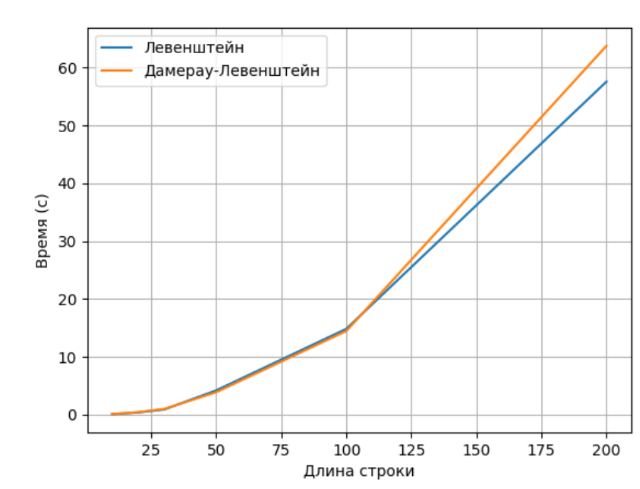
\includegraphics[width=130mm]{inc/img/timing.png}
    \caption{Сравнение времени работы алгоритма поиска расстояния Левенштейна и Дамерау-Левенштейна}
    \label{img:timing}
\end{figure}







\section*{Вывод}

В результате эксперимента было получено, что на случайных данных, алгоритм Дамерау-Левенштейна работает быстрее алгоритма Левенштейна. Например при длине строки в 200 символов алгоритм Дамерау-Левенштейна работает на 10$\%$ быстрее алгоритма Левенштейна. Также в результате эксперимента было получено, что при длине строки меньше 100 символов алгоритмы работают за одинаковое время. Можно сделать вывод, что при размерности строк > 100 символов лучше использовать алгоритм Дамерау-Левенштейна.